\documentclass[aspectratio=169,12pt]{beamer}

% Presentation slides for lecture_notes.tex (the companion document has the details)

% ---------------------------------------------------------------------------
% Theme: metropolis with Fira Sans (pdflatex-compatible), navy/amber palette
% ---------------------------------------------------------------------------
\usetheme[progressbar=frametitle, numbering=fraction, block=fill, sectionpage=progressbar]{metropolis}
\usepackage[sfdefault]{FiraSans}
\usepackage{FiraMono}
\usefonttheme[onlymath]{serif}

\definecolor{navy}{HTML}{1F3A5F}
\definecolor{amber}{HTML}{E09F3E}
\definecolor{paper}{HTML}{FAFAF7}
\definecolor{ink}{HTML}{23262B}
\definecolor{zero}{HTML}{DCEFE0}
\definecolor{finite}{HTML}{FCEBC9}
\definecolor{diverge}{HTML}{F6D5D1}

\setbeamercolor{normal text}{fg=ink, bg=paper}
\setbeamercolor{frametitle}{fg=white, bg=navy}
\setbeamercolor{progress bar}{fg=amber, bg=navy!30}
\setbeamercolor{title separator}{fg=amber}
\setbeamercolor{alerted text}{fg=amber!85!black}
\setbeamercolor{block title}{fg=white, bg=navy}
\setbeamercolor{block body}{fg=ink, bg=navy!6}
\setbeamercolor{section in toc}{fg=navy}

\usepackage{amsmath, amssymb}
\usepackage{booktabs}
\usepackage{array}
\usepackage{colortbl}
\usepackage{tikz}
\usetikzlibrary{arrows.meta, positioning, calc, decorations.pathreplacing}

\tikzset{
  >={Latex[length=1.6mm, width=1.3mm]}, thick, draw=navy,
  block/.style = {draw=navy, fill=navy!6, rounded corners=2pt, minimum height=2.3em, minimum width=4.2em},
  sum/.style   = {draw=navy, circle, inner sep=0pt, minimum size=1.1em},
}

\title{Steady-State Error}
%\subtitle{Where does the output end up?}
\author{ME 2801}% \quad\textbar\quad Fall 2026}
\date{}
%\date{Details and derivations: \emph{Steady-State Error: Lecture notes}}

\begin{document}

\maketitle


\begin{frame}{Two performance questions}
  Transient performance quantifies speed; \\
  steady-state performance quantifies accuracy.

  \bigskip
  \begin{columns}[T]
    \column{0.45\textwidth}
    \begin{block}{Transient: \emph{how} it gets there}
      Settling time, overshoot\\
      Damping ratio\\
      Pole locations
    \end{block}
    \column{0.45\textwidth}
    \begin{block}{Steady state: \emph{where} it ends up}
      Final offset, ramp lag\\
      Persistent tracking error\\
      DC behavior of the loop
    \end{block}
  \end{columns}
\end{frame}

\begin{frame}{Example: pointing a satellite}
  \begin{columns}[c]
    \column{0.42\textwidth}
    \centering
    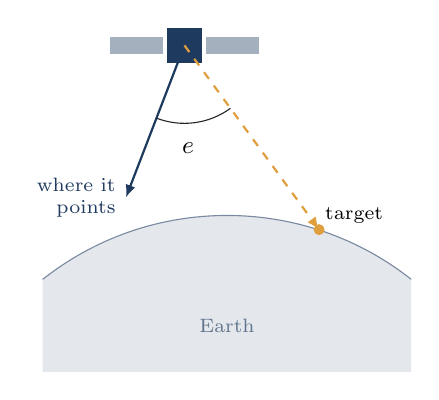
\begin{tikzpicture}[scale=0.9]
      % Earth
      \begin{scope}
        \clip (-2.6,-2.2) rectangle (2.6,0.2);
        \fill[navy!12] (0,-4.2) circle (4.2);
        \draw[navy!60] (0,-4.2) circle (4.2);
      \end{scope}
      \node[navy!70, font=\scriptsize] at (0,-1.55) {Earth};
      % ground target
      \coordinate (tgt) at (1.3,-0.2);
      \fill[amber] (tgt) circle (2.2pt);
      \node[above right, font=\scriptsize, inner sep=2pt] at (tgt) {target};
      % satellite: body + solar panels
      \coordinate (sat) at (-0.6,2.4);
      \fill[navy!40] ($(sat)+(-1.05,-0.12)$) rectangle ($(sat)+(-0.3,0.12)$);
      \fill[navy!40] ($(sat)+(0.3,-0.12)$) rectangle ($(sat)+(1.05,0.12)$);
      \fill[navy] ($(sat)+(-0.25,-0.25)$) rectangle ($(sat)+(0.25,0.25)$);
      % boresight (current) and line of sight (desired)
      \draw[->, navy, thick] (sat) -- ($(sat)!2.3cm!(-1.6,-0.2)$) node[left, font=\scriptsize, align=right] {where it\\points};
      \draw[->, amber, thick, dashed] (sat) -- (tgt);
      % pointing error angle
      \draw[ink, thin] ($(sat)!1.1cm!(-1.6,-0.2)$) arc[start angle={atan2(-2.6,-1.0)}, end angle={atan2(-2.6,1.9)}, radius=1.1cm];
      \node[font=\small] at ($(sat)+(0.05,-1.45)$) {$e$};
    \end{tikzpicture}

    \column{0.55\textwidth}
    \centering
    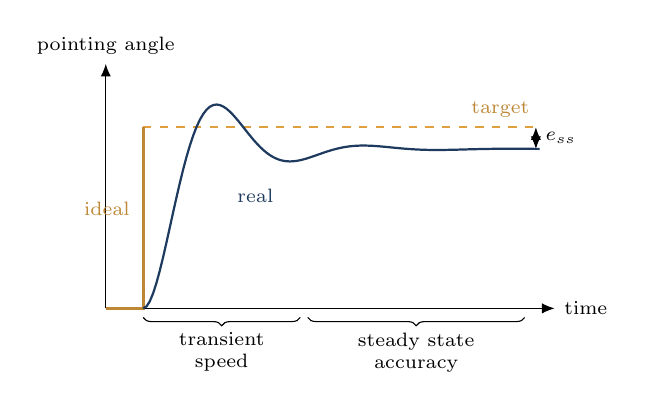
\begin{tikzpicture}[xscale=0.95, yscale=2.3]
      % axes
      \draw[->, thin] (0,0) -- (6.0,0) node[right, font=\scriptsize] {time};
      \draw[->, thin] (0,0) -- (0,1.35) node[above, font=\scriptsize] {pointing angle};
      % reference
      \draw[amber, thick, dashed] (0.5,1) -- (5.8,1) node[above left, font=\scriptsize, text=amber!85!black] {target};
      % ideal: instant and exact
      \draw[amber!85!black, very thick] (0,0) -- (0.5,0) -- (0.5,1);
      \node[font=\scriptsize, text=amber!85!black, anchor=east] at (0.45,0.55) {ideal};
      % real: transient, then a steady-state offset
      \draw[navy, thick, domain=0:5.3, samples=120]
        plot ({0.5+\x}, {0.88*(1 - exp(-1.3*\x)*(cos(deg(3.2*\x)) + 0.4*sin(deg(3.2*\x))))});
      \node[font=\scriptsize, text=navy] at (2.0,0.62) {real};
      % annotations
      \draw[<->, thin] (5.75,0.88) -- (5.75,1) node[midway, right, font=\scriptsize] {$e_{ss}$};
      \draw[decorate, decoration={brace, amplitude=3pt, mirror}, thin] (0.5,-0.05) -- (2.6,-0.05) node[midway, below=2pt, font=\scriptsize, align=center] {transient\\\alert{speed}};
      \draw[decorate, decoration={brace, amplitude=3pt, mirror}, thin] (2.7,-0.05) -- (5.6,-0.05) node[midway, below=2pt, font=\scriptsize, align=center] {steady state\\\alert{accuracy}};
    \end{tikzpicture}
  \end{columns}

  \bigskip
  \centering Ideal Response: Intantaneous and exact. \\
  Real Response: always a \alert{tradeoff}.
\end{frame}

\begin{frame}{Setting and assumptions}
  \begin{center}
  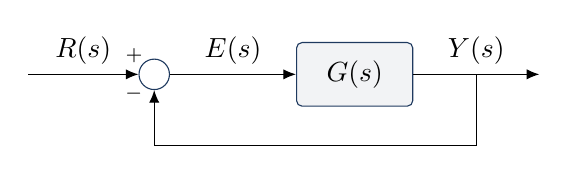
\begin{tikzpicture}
    \node[coordinate]                   (rin)  {};
    \node[sum,   right=1.4cm of rin]    (sum)  {};
    \node[block, right=1.6cm of sum]    (G)    {$G(s)$};
    \node[coordinate, right=1.6cm of G] (yout) {};
    \node[font=\scriptsize, inner sep=0pt, anchor=south east] at (sum.north west) {$+$};
    \node[font=\scriptsize, inner sep=0pt, anchor=north east] at (sum.south west) {$-$};
    \draw[->] (rin) -- node[above]{$R(s)$} (sum);
    \draw[->] (sum) -- node[above]{$E(s)$} (G);
    \draw[->] (G)   -- node[above]{$Y(s)$} (yout);
    \coordinate (fbk) at ($(G.east)!0.5!(yout)$);
    \draw[->] (fbk) -- ++(0,-0.9) -| (sum.south);
  \end{tikzpicture}
  \end{center}

  \begin{itemize}
    \item Unity negative feedback, with foward (open-loop) path $G(s) = C(s)\,P(s)$
    \item Stability first - must be stable to asses the steady-state error.
    \item Error is formed at the summing junction: $E(s) = R(s) - Y(s)$
  \end{itemize}

  \small Note: elsewhere $G(s)$ often means the plant alone. Here it is the whole forward path.
\end{frame}

\begin{frame}{Master equation: error transfer function + final value theorem}
  From $Y = G\,E$ and $E = R - Y$:
  \[
    E(s) = \frac{R(s)}{1+G(s)}
    \qquad\Longrightarrow\qquad
    e(\infty) = \lim_{s\to 0} s\,E(s)
  \]

  \begin{center}
  \colorbox{navy!8}{\parbox{0.5\textwidth}{\centering\vspace{0.4em}
    $\displaystyle e(\infty) = \lim_{s\to 0}\,\frac{s\,R(s)}{1+G(s)}$
  \vspace{0.4em}}}
  \end{center}

  \medskip
  Everything else a special case:
  \begin{itemize}
    \item Given foward loop (controller and plant)
    \item Choose an input $R(s)$ (step, ramp, parabola)
    \item Evaluate the steady-state error 
  \end{itemize}
\end{frame}

% ===========================================================================
\section{Inputs and system type}
% ===========================================================================

\begin{frame}{Three test inputs}
  \begin{center}
  \renewcommand{\arraystretch}{1.3}
  \begin{tabular}{lccl}
    \toprule
    Input    & $r(t)$         & $R(s)$  & Scenario \\
    \midrule
    Step     & $1$            & $1/s$   & Hold a fixed setpoint \\
    Ramp     & $t$            & $1/s^2$ & Track a constant-velocity target \\
    Parabola & $\tfrac12 t^2$ & $1/s^3$ & Track an accelerating target \\
    \bottomrule
  \end{tabular}
  \end{center}

  \bigskip
  Stationary target $\rightarrow$ constant-velocity target $\rightarrow$ maneuvering target.

  Each step up needs \alert{one more integrator} in the forward path (controller + plant) to keep the error bounded.
\end{frame}

\begin{frame}{System type}
  \[
    G(s) = \frac{K\,(s+z_1)(s+z_2)\cdots}{s^{\alert{n}}\,(s+p_1)(s+p_2)\cdots}
  \]

  \begin{center}
  Type $n$ = number of pure integrators (poles at $s = 0$) in $G(s)$
  \end{center}

  \bigskip
  \begin{itemize}
    \item A property of the \emph{combined} path $C(s)P(s)$, not the plant alone
    \item Adding $K_I/s$ to the controller raises the type by one
    \item It does not matter where the integrator lives, only that it is in the loop
  \end{itemize}
\end{frame}

% ===========================================================================
\section{Error constants and the diagonal}
% ===========================================================================

\begin{frame}{Static error constants}
  Three limits appear so often they get names:
  \begin{align*}
    K_x &= \lim_{s\to 0} G(s)      && \text{position} \\[2pt]
    K_v &= \lim_{s\to 0} s\,G(s)   && \text{velocity} \\[2pt]
    K_a &= \lim_{s\to 0} s^2\,G(s) && \text{acceleration}
  \end{align*}

  \bigskip
  \small We write $K_x$ rather than the textbook $K_p$, to avoid confusion with the PID gain $K_P$.
\end{frame}

\begin{frame}{The diagonal pattern}
  \begin{columns}[c]
    \column{0.52\textwidth}
    \centering
    \renewcommand{\arraystretch}{2.0}
    \setlength{\tabcolsep}{4pt}
    \begin{tabular}{l>{\centering\arraybackslash}p{1.5cm}>{\centering\arraybackslash}p{1.5cm}>{\centering\arraybackslash}p{1.5cm}}
               & Type 0 & Type 1 & Type 2 \\
      Step     & \cellcolor{finite}$\dfrac{1}{1+K_x}$ & \cellcolor{zero}$0$ & \cellcolor{zero}$0$ \\
      Ramp     & \cellcolor{diverge}$\infty$ & \cellcolor{finite}$\dfrac{1}{K_v}$ & \cellcolor{zero}$0$ \\
      Parabola & \cellcolor{diverge}$\infty$ & \cellcolor{diverge}$\infty$ & \cellcolor{finite}$\dfrac{1}{K_a}$ \\
    \end{tabular}

    \column{0.44\textwidth}
    \small
    \begin{itemize}
      \item[\textcolor{zero!60!black}{$\blacksquare$}] Above the diagonal: zero error (more than enough integrators)
      \item[\textcolor{finite!60!black}{$\blacksquare$}] On the diagonal: finite error, set by the matching constant
      \item[\textcolor{diverge!60!black}{$\blacksquare$}] Below the diagonal: error diverges (not enough integrators)
    \end{itemize}
  \end{columns}
\end{frame}

\begin{frame}{One number, four facts}
  A specification of \alert{$K_v = 20$} tells us:
  \begin{enumerate}
    \item The closed loop is stable
    \item The loop is Type 1 (only Type 1 has a finite, nonzero $K_v$)
    \item The relevant input is a ramp
    \item The ramp error is $1/K_v = 5\%$ per unit slope
  \end{enumerate}
\end{frame}

\begin{frame}{Design recipe}
  When the type is fixed and only a forward gain $K$ is free:
  \begin{enumerate}
    \item Identify the type by inspection
    \item Write the relevant constant ($K_x$, $K_v$ or $K_a$) in terms of $K$
    \item Solve for $K$ to meet the spec
    \item \alert{Check that the closed loop is still stable at that $K$}
  \end{enumerate}
\end{frame}

% ===========================================================================
\section{Removing steady-state error}
% ===========================================================================

\begin{frame}{Two ways to remove steady-state error}
  \begin{center}
  \small
  \renewcommand{\arraystretch}{1.35}
  \begin{tabular}{@{}l>{\raggedright\arraybackslash}p{4.6cm}>{\raggedright\arraybackslash}p{4.6cm}@{}}
    \toprule
                   & \textbf{Integrator (PI)}       & \textbf{Feedforward $1/K_{\mathrm{dc}}$} \\
    \midrule
    Mechanism      & Accumulates error until $e \to 0$ & Supplies the steady-state effort \\
    Needs a model? & No, self-correcting            & Yes, the plant DC gain \\
    System type    & $+1$                           & Unchanged \\
    Disturbances   & Rejects them                   & Does not see them \\
    Cost           & Slower, overshoot, windup      & Residual error if model is wrong \\
    \bottomrule
  \end{tabular}
  \end{center}
\end{frame}

\begin{frame}{Why the integrator works}
  At steady state in a stable loop, every signal is constant:
  \[
    \dot u_I = K_I\, e = 0 \quad\Longrightarrow\quad e = 0
  \]

  The integrator keeps adding to the input as long as the output is short, and settles at exactly the bias the plant needs.

  \bigskip
  \begin{block}{Best of both: PI + feedforward}
    Feedforward delivers most of the effort immediately; the integrator corrects whatever the model got wrong. Speed \emph{and} robustness.
  \end{block}
\end{frame}

\begin{frame}{Takeaways}
  \begin{itemize}
    \item One limit, $\lim_{s\to 0} s\,R(s)/(1+G(s))$, produces the whole table
    \item Stability is the silent precondition
    \item Type belongs to $G = CP$: P on a Type 0 plant is Type 0; PI on the same plant is Type 1
    \item Higher type is not free: each integrator costs stability margin
    \item Feedforward bypasses the error junction, so it sits outside the master equation
  \end{itemize}
\end{frame}

\end{document}
